\section{Experimental setup}
% TODO: fixa röda tråden mellan metoden och utförandet.

The experimental setup used to measure the index of refraction for various gases is illustrated in Fig. \ref{fig:experimentalSetup}. The HeNe-laser beam is divided into two legs, reference leg $L_1$ and signal leg $L_2$ via a beam splitter (BS). The beam travelling down the signal leg is transmitted through a gas chamber made of acryllic glas, with inner length $d=100(1)$ mm. And then reflected via a mirror back the same way where it is reflected on the beam splitter where it coincides with the other part which has been reflected in $L_1$. The recombined laser beam shines through a small apperature in order to elliminate laser beams due to unwanted reflections. It then reaches a lens which diverges the laser beam in order to increase the resolution. A photodiode is mounted after the lens in order to pick up any changes of incident intensity of the combined laser beam. In order to eliminate ethalons inside the gas chamber, it was mounted at an angle relative the incident laser beam.

\begin{figure}[H]
  \centering
  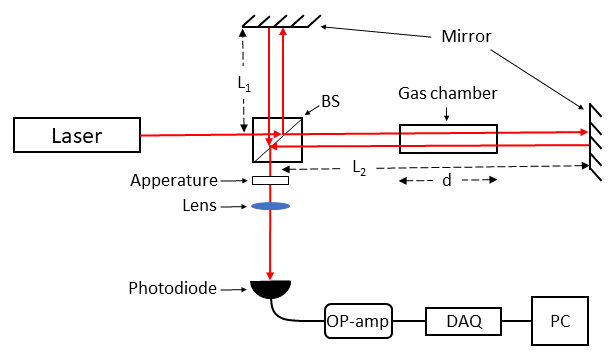
\includegraphics[width=0.8\textwidth]{Exp_setup.png}
  \caption{Experimental setup. The laser beam is split into two rays at the beam splitter. One ray propagates in the reference leg (L$_1$) and is reflected back to the beam splitter. The other ray that was split at the beam splitter, propagates in to the signal leg (L$_2$) via a gas chamber to a mirror and reflected back the same way to the beam splitter. The two rays coincide at the beam splitter again and propagates through an apperature and a lens and illuminates a photodiode. The two rays will interfere with eachother and an interferance pattern will emerge.}
  \label{fig:experimentalSetup}
\end{figure}

The photodiode is connected to an operational amplifier with low pass filter in order to amplify the signal and reduce noise in the circut. The data acquisition card (DAQ) retrives the amplified signal from the photodiode as well as a signal from an instrument measuring the pressure inside the gas chamber. The data is captured via LabView and analyzed in MATLAB.

In order to convert the voltage accuired from the pressure measurment into pressure, it had to be calibrated. The calibration curve is shown in Fig. \ref{fig:calibration}. The linear fit on the calibration measurement was calculated in by linear least squares in MATLAB, the fitted line has the equation $P = 12.5(2)V+25.6(1)$. 


\begin{figure}[H]
  \centering
  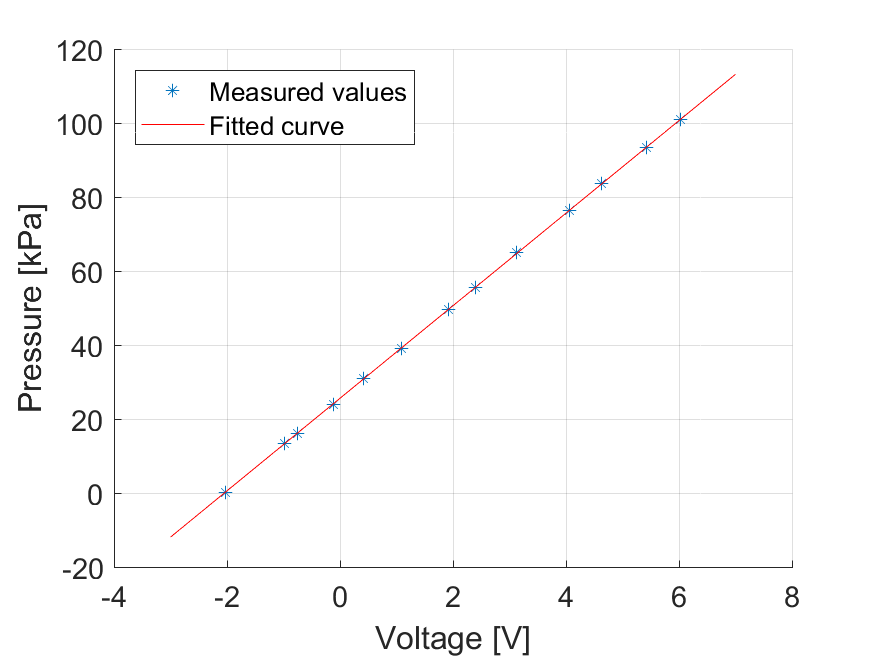
\includegraphics[width=0.8\textwidth]{matlab/calibration.png}
  \caption{Calibration curve for voltage to pressure relation. The fitted line is $P = 12.5(2)V+25.6(1)$.}
  \label{fig:calibration}
\end{figure}

The two legs were are aligned propertly in order to see a interference pattern at the photodiode with high resolution and contrast. By filling the gas chamber with one of the gases of intrest (air, helium, argon or nitrogen), from vaccum and measuring the change of intensity at the photodiode as well as the pressure in the gas chamber continuously. By counting the fringes (seen as peaks from the photodiode). The index of refraction could be calculated via Eq. \ref{eq:refrVaccum} and Eq. \ref{eq:slope}.

%, an interferance pattern will emerge on the photodiode. If vaccum is created inside the gas chamber and then a steady flow of gas added, the optical path will increase. An interferance pattern (fringes) on the photodiode  will start to move continuously. By measuring the intensity changes on the photodiode and relating this to the pressure change in the gas chamber, one can calculate the index of refraction via Eq. \ref{eq:refrVaccum} and Eq. \ref{eq:slope}.



In order to estimate the error of $a =\Delta N/ \Delta P$ from Eq. \ref{eq:slope}, the errors of $\Delta N$ ($S_{\Delta N}$) and $\Delta P$ ($S_{\Delta P}$) has to be estimated. These errors was estimated to $S_{\Delta N}=0.5$ and $S_{\Delta P}=0.1$ kPa. By fitting the two lines that are inside these errors for all measurements. The slopes of these lines will generate a confidence interval for $a$.
